\setcounter{page}{2}

\addchap{Цель работы}

Изучение основ построения микропроцессорных систем на ПЛИС. В
ходе работы необходимо ознакомиться с принципами построения систем
на кристалле (СНК) на основе ПЛИС, получить навыки проектирования
СНК в САПР Altera Quartus II, выполнить проектирование и верификацию
системы с использованием отладочного комплекта Altera DE1Board.

\chapter{Функциональная схема разрабатываемой системы на кристалле}

Представлена на рис. 1.1.
\begin{figure}[H]
	\begin{center}
		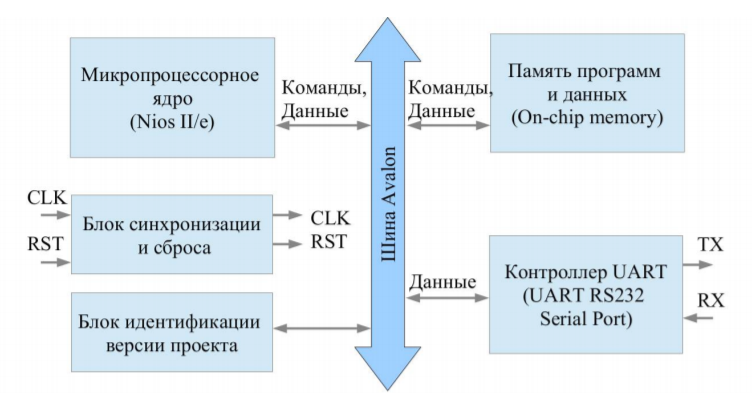
\includegraphics[scale=0.6]{assets/scheme.png}
	\end{center}
	\caption{Функциональная схема разрабатываемой системы на кристалле}
\end{figure}

Она состоит из следующих элементов:
\begin{enumerate}
	\item микропроцессорное ядро Nios II/e, выполняющее функции управления системой;
	\item внутренняя оперативная память СНК, используемая для хранения программы управления и данных;
	\item системная шина Avalon, обеспечивающая связность всех компонентов системы;
	\item блок синхронизации и сброса, обеспечивающий обработку входных сигналов сброса и синхронизации и распределение их в системе. Внутренний сигнал сброса синхронизирован и имеет необходимую для системы длительность;
	\item блок идентификации версии проекта, обеспечивающий хранение и выдачу уникального идентификатора версии, который используется программой управления при инициализации системы;
	\item контроллер UART, обеспечивающий прием и передачу информации по интерфейсу RS232.
\end{enumerate}

\chapter{Создания модуля системы на кристале QSYS}

В процессе были выполнены следующие действия:
\begin{itemize}
	\item создан новый модуль QSYS;
	\item установлена частота внешнего сигнала синхронизации 50 000 000 Гц;
	\item добавлены в проект модуль синхронизируемого микропроцессорного ядра Nios2 и модуль ОЗУ программ и данных;
	\item добавлены компоненты Avalon System ID, Avalon UART;
	\item создана сеть синхронизации и сбоса системы;
	\item сигналы TX и RX экспортированы во внешние порты;
	\item назначены базовые адреса устройств.
\end{itemize}

Сделанный модуль системы представлен на рис. 2.1.
\begin{figure}[H]
	\begin{center}
		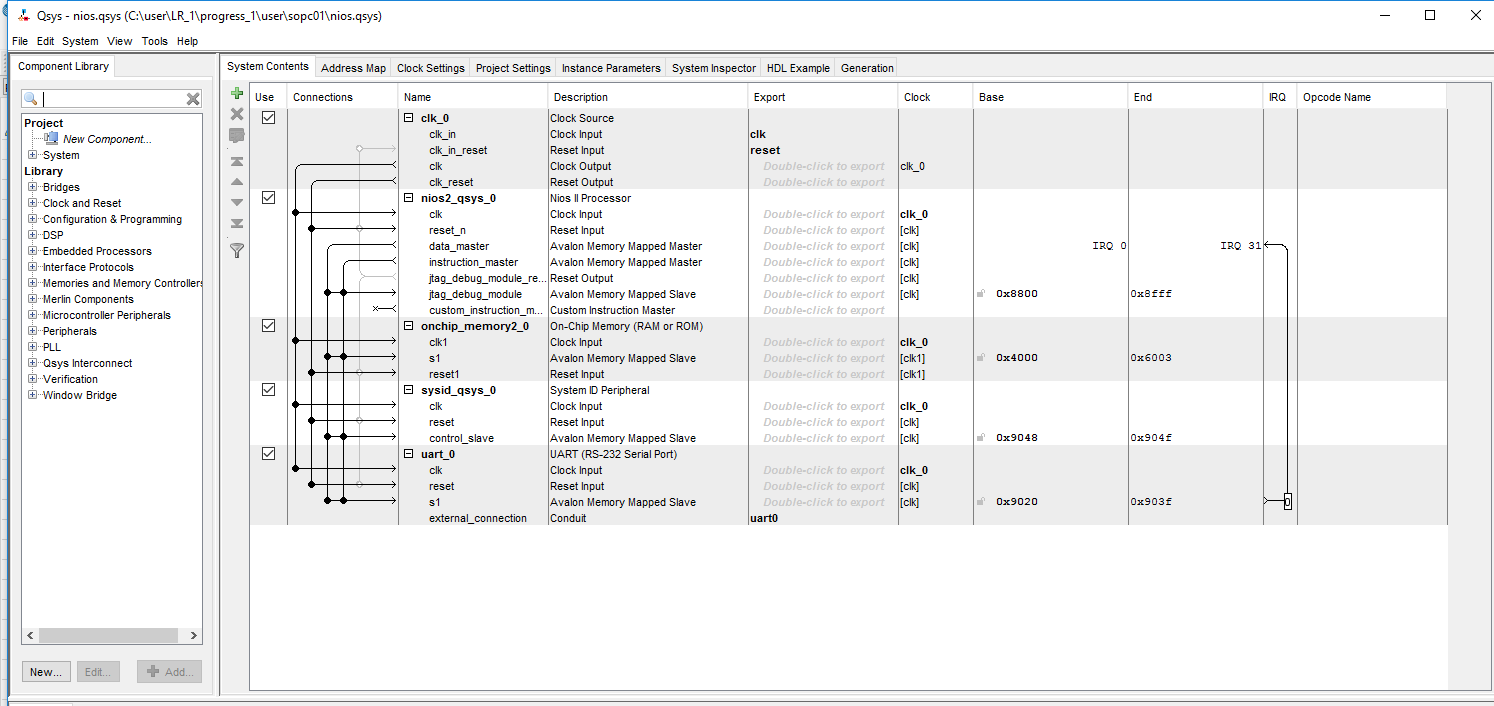
\includegraphics[scale=0.5]{assets/qsys.png}
	\end{center}
	\caption{Готовый модуль в системе проектирования системы на кристалле Altera Qsys}
\end{figure}

\chapter{Назначение портам контактов микросхемы}

В соответствии с методическими указанями к лабораторной сигналам были назначены следующие контакты:
\begin{itemize}
	\item clk - контакт L1;
	\item reset - контакт R22;
	\item uart0\_{rxd} - контакт F14;
	\item uart0\_{txd} - контакт G12.
\end{itemize}

Результат представлен на рис. 3.1.
\begin{figure}[H]
	\begin{center}
		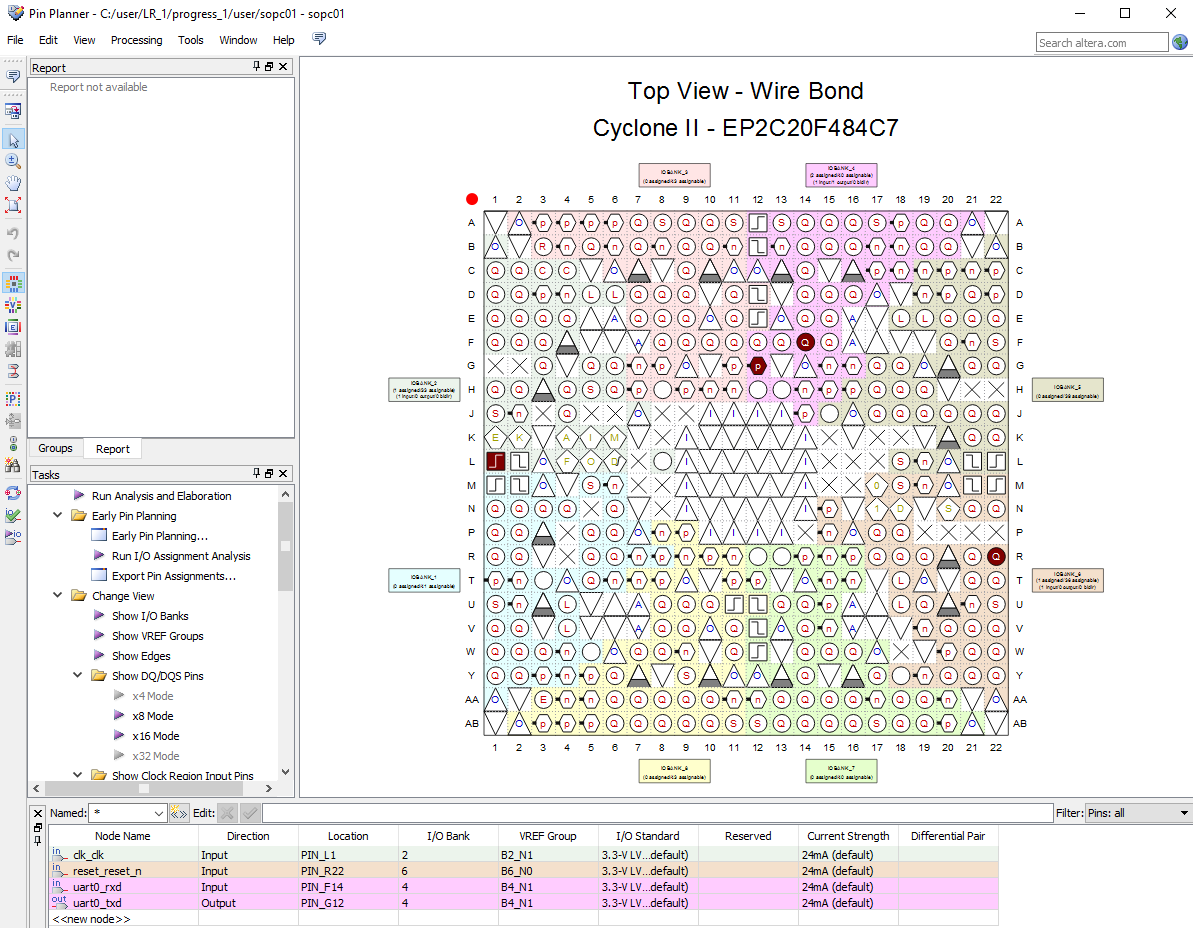
\includegraphics[scale=0.5]{assets/pin_planner.png}
	\end{center}
	\caption{Модуль Pin Planner}
\end{figure}

\chapter{Создание проекта Nios2}

Был создан файл эхо-программы приема-передачи по интерфейсу R32. Его листинг представлен ниже. Также был создан образ ОС HAL с драйверами устройств, используемых в аппаратном проекте.

\captionsetup{singlelinecheck = false, justification=raggedright}
\begin{lstlisting}[label=code, caption=Код рассматриваемой программы]
#include "sys/alt_stdio.h"
#include "system.h"
#include "altera_avalon_sysid_qsys.h"
#include "altera_avalon_sysid_qsys_regs.h"
int main()
{ 
	char ch;
	alt_putstr("Hello from System on Chip\n");
	alt_putstr("Send any character\n");

	  int id = IORD_ALTERA_AVALON_SYSID_QSYS_ID(SYSID_QSYS_O_BASE);
  	  char arr[10];
  	  int i = 0;
  	  while (i <= 3) {
  		  arr[3-i] = (char)('0' + id%10);
  		  id = id/10;
  		  i = i+1;
  	  }
  	  arr[4] = '\0';
  	  alt_putstr(arr);
  while (1) {
	  ch=alt_getchar();
	  alt_putchar(ch);
  }
  return 0;
}
\end{lstlisting}
\captionsetup{singlelinecheck = false, justification=centering}

\chapter{Подключение к ПК отладочной платы}

К ПК была подключена отладочная плата с ПЛИС EPC2C20. Была выполнена верификация проекта с использованием программы терминала. Вывод сообщения с номером группы и вариантом представлен на рис. 5.1.
\begin{figure}[H]
	\begin{center}
		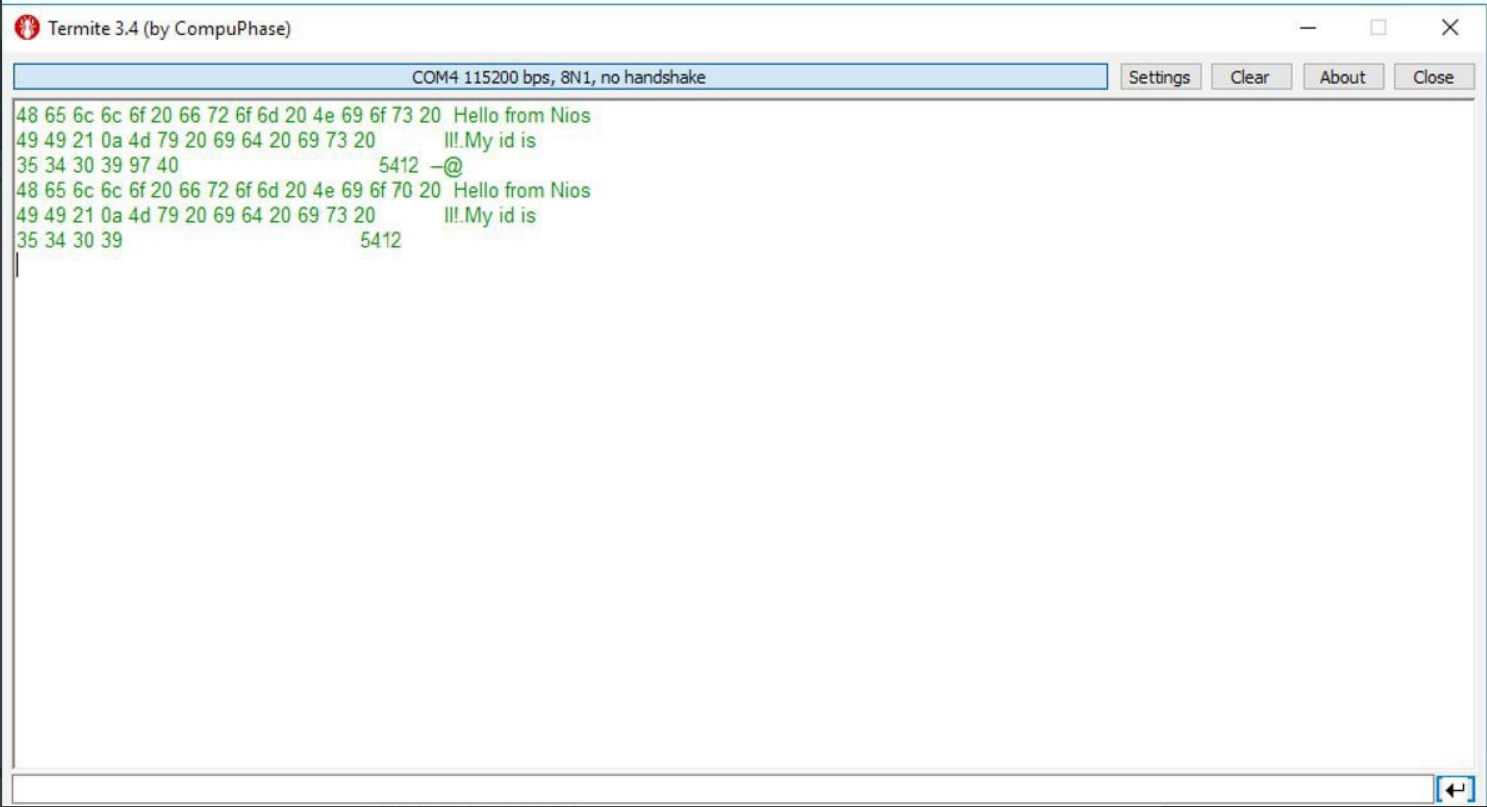
\includegraphics[scale=0.42]{assets/view.png}
	\end{center}
	\caption{Тестирование}
\end{figure}

\addchap{Вывод}

В ходе данной лабораторной работы были изучены основы построения
микропроцессорных систем на ПЛИС, получены навыки проектирования
СНК в САПР Altera Quartus II, также были выполнены проектирование
и верификация системы с использованием отладочного комплекта Altera
DE1Board. Поставленная цель была достигнута. 